\chapter{粒子、波与分辨的能量}

\section{粒子还是场？}

粒子物理学研究的是什么？粒子---但这一回答立刻引出一个古老的问题。自然界是离散的吗？这里的离散意味着物质由彼此分离、不可分割的单元组成，而不是说它圆滑得体。希腊词\emph{atom}意为不可分割，尽管如今称为原子的物体可以被分开。目前，\emph{粒子}将作为离散单元的统称。

与之对立的图景是连续统。此时物质不是分离碎片的集合，而是连续地弥散于空间之中。它的自然语言是场的语言。场是位置的函数：材料的密度是一个场，电场和磁场也是场。后者决定带电粒子如何运动，但场本身在经典意义上被设想为连续分布于空间之中。

不应过分拘泥于这些观念的历史顺序。这一顺序之所以有用，是因为它展示了论证的逻辑，而不是因为它提供了可靠的年表。粒子词汇包括原子、分子、碰撞和局域物体；连续统词汇包括场和连续变化的属性。哪一幅图景是正确的？量子力学使两者都不可能完全正确，但它也使两者都不可能完全错误。

讨论将部分地自足，尽管后面的论证会用到量子力学、经典力学、狭义相对论和电磁学。眼下的问题仍然更简单：最初是什么使人们相信物质确实是离散的？

\section{物质离散性的化学证据}

至少在这一逻辑叙述中，最早的严肃证据来自化学而非物理学。这一区分是人为的：化学在很大程度上就是原子和分子的物理学。道尔顿比较了不同物质相同数目分子的质量。确定样品含有相同数目本身就是一大难题。阿伏伽德罗的名字在此登场，而一摩尔就是阿伏伽德罗数个分子。仅仅为了比较含有相同分子数的样品，并不需要该数目的实际值。

引人注目的规律是，摩尔质量近似地以氢的摩尔质量的整数倍出现。乘数一般不是\(3/2\)、\(\pi\)或任意实数，而是接近整数的数。例如碳-12大约带有十二个以氢为代表的质量单位。这强烈暗示物质由质量几乎相同的重复构建单元构成。

现代解释消除了这一奥秘。普通原子包含质子、中子和电子。电子的质量大约只有质子或中子质量的两千分之一，因此电子对原子质量的贡献很小。质子和中子几乎承载了全部质量，而它们的质量相差远小于百分之一。由于普通氢的原子核就是一个质子，原子或分子的质量近似为氢尺度核质量的整数倍。这一陈述只是近似的：质子和中子的质量并不相同，电子也有少许贡献。然而，这种近整数规律揭示了离散的组成部分。

分子随后被理解为原子的组合。十九世纪的化学识别出大约一百种原子，并将它们组织为元素；在基本计数中大约有九十二种天然存在，一旦计入同位素还会有更多区分。周期表并非朴素意义上简单重复相等区块的周期表，但它组织了这些彼此分离的物种。在那个阶段，元素本身看起来就像是基本构建单元。爱因斯坦1905年的工作提供了一种定量方式，以远为决定性的方式确立物质的分子理论，但化学证据已经使原子图景令人信服。

临近十九世纪末，这一表面上的终点失效了。电子被发现，放射性揭示了元素即基本单元这一图景无法容纳的现象。放射性已经以微缩的形式包含了后来成为核物理和粒子物理的许多问题。

\section{放射性与分离束}

确切的归属和时间顺序并不确定。贝克勒尔暂时与这样一个观察相关联：放射性物质恰好位于照相底片附近，并对其产生了影响，仿佛有不可见的辐射照射了它。与其仅仅把被雾化的底片视为损坏，人们可以问是什么到达了底片。玛丽·居里后来大量的工作也属于这段历史，但早期发现的精确划分对于实验逻辑而言并不需要。

把材料放在致密铅块的深处，并留出一条通向照相底片的狭窄通道。铅之所以有用，是因为它致密，而通道则对逃逸出来的东西进行准直。底片不是形成弥散的曝光，而是显出一个局域化的斑点，暗示存在一束有方向的射线。在这种逻辑意义上，这是第一束粒子束，尽管在这个阶段这束射线的性质尚不清楚。

现在让准直后的发射通过一个垂直于轨迹平面的磁场。曝光分成三支。一支继续不偏转。两支向相反方向弯曲，而且弯曲量不相等。当电荷的符号反转时，磁力方向也反转，因此向相反方向弯曲的两支表现为带相反电荷的辐射；直行的那一支表现为中性辐射。\footnote{该示意图重建了讲座视频中在00:14:34和00:19:31之间绘制的图。}

\begin{figure}[h]
\centering
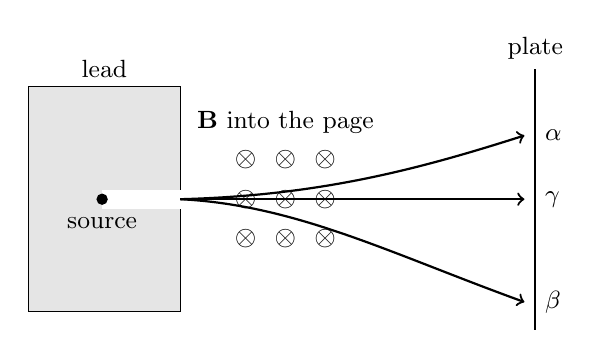
\begin{tikzpicture}[scale=0.92]
\draw[fill=gray!20] (0,-1.55) rectangle (2.1,1.55);
\draw[fill=white,draw=none] (1.02,-0.13) rectangle (2.12,0.13);
\draw[fill=black] (1.02,0) circle (0.07);
\node[below] at (1.02,-0.12) {\small source};
\node[above] at (1.05,1.55) {\small lead};
\foreach \x in {3.0,3.55,4.1}
  \foreach \y in {-0.55,0,0.55}
    \node at (\x,\y) {\(\otimes\)};
\node[above] at (3.55,0.78) {\small \(\mathbf B\) into the page};
\draw[thick] (7,-1.8) -- (7,1.8);
\node[above] at (7,1.8) {\small plate};
\draw[thick,->] (2.1,0) -- (6.85,0);
\draw[thick,->] (2.1,0) .. controls (4.0,0.05) and (5.35,0.40) .. (6.85,0.88);
\draw[thick,->] (2.1,0) .. controls (3.7,-0.08) and (5.0,-0.75) .. (6.85,-1.42);
\node[right] at (7,0.88) {\small \(\alpha\)};
\node[right] at (7,0) {\small \(\gamma\)};
\node[right] at (7,-1.42) {\small \(\beta\)};
\end{tikzpicture}
\caption{横向磁场中的准直放射性射线。中性成分不偏转，而带相反电荷的成分向相反方向弯曲，且弯曲量不相等。}
\end{figure}

这三种成分被命名为{\proseunicodefont α}、{\proseunicodefont β}和{\proseunicodefont γ}。用现代术语来说，
\begin{equation}
\begin{aligned}
\beta\text{-radiation} &= \text{electrons},\\
\alpha\text{-radiation} &= \text{helium nuclei},\\
\gamma\text{-radiation} &= \text{photons}.
\end{aligned}
\end{equation}
一个{\proseunicodefont α}粒子包含两个质子和两个中子，这解释了它的质量数为4。在道尔顿近似的整数序列中，氦因此会占据第4号：四个氢尺度的核单位。{\proseunicodefont β}射线是已经在阴极射线实验中知道的带负电的电子。{\proseunicodefont γ}射线不带电荷。

当源足够稀薄，并且探测器能够分辨单个到达事件时，看起来连续的曝光就变成了一系列分离的事件：滴答、滴答、滴答。对{\proseunicodefont β}、{\proseunicodefont α}和{\proseunicodefont γ}辐射也可以这样做。盖革计数器给出了正确的图景，无论最早的装置是否正是在那种条件下运行的。每种成分都以离散的束到达。{\proseunicodefont γ}仍然是谜：它是中性的，却被一次一个事件地探测到。{\proseunicodefont γ}辐射是能量非常高的光，而普朗克、尤其是爱因斯坦把光与量子联系起来。然而，在直面那个结论之前，必须认真对待光是波的经典证据。

\section{光的经典波动性质}

在经典意义上，光是连续性的最强例子。它由作为连续波传播的电场和磁场组成。牛顿曾倾向于微粒图景，但波动实验取代了它。摇动一个电荷会产生电磁辐射。宏观天线可以发射无线电波、微波、红外线、可见光或紫外辐射；电荷在原子内部运动时也是一根天线。发射出的辐射可以使照相底片曝光。

单个开口给出了波动行为的第一个迹象。如果光是子弹流，那么小开口预期会形成一个锐利准直的斑点。相反，照明扩展成一个模糊区域。然而，仅凭扩展并不具有决定性，因为人们可以想象粒子被孔径边缘处的力偏转。

两个开口产生更尖锐的检验。两束独立的粒子流会给出两个重叠的涂抹，也许在它们重叠处最亮。波则做不同的事。来自一个开口的波峰可以遇到来自另一个开口的波峰并增强它；波峰也可以遇到波谷并抵消它。因此屏幕上显示出交替的明带和暗带，包括单独任一开口都会照亮的暗处。\footnote{该示意图重建了讲座视频中在00:25:00和00:29:49之间绘制的孔径和干涉图。}

\begin{figure}[h]
\centering
\resizebox{\linewidth}{!}{%
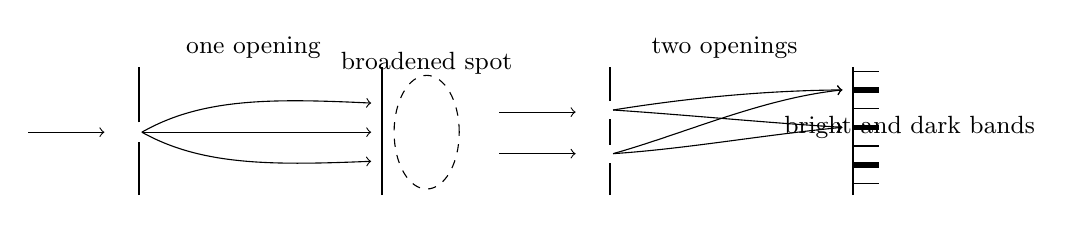
\begin{tikzpicture}[scale=0.88]
\begin{scope}
\draw[->] (-0.3,1.06) -- (0.8,1.06);
\draw[thick] (1.3,0.15) -- (1.3,0.92);
\draw[thick] (1.3,1.20) -- (1.3,2.0);
\draw[thick] (4.8,0.15) -- (4.8,2.0);
\draw[->] (1.34,1.06) .. controls (2.2,1.55) and (3.2,1.55) .. (4.65,1.48);
\draw[->] (1.34,1.06) -- (4.65,1.06);
\draw[->] (1.34,1.06) .. controls (2.2,0.58) and (3.2,0.58) .. (4.65,0.64);
\draw[dashed] (5.45,1.06) ellipse (0.47 and 0.82);
\node at (2.95,2.28) {\small one opening};
\node at (5.45,2.05) {\small broadened spot};
\end{scope}
\begin{scope}[xshift=6.8cm]
\draw[->] (-0.3,1.35) -- (0.8,1.35);
\draw[->] (-0.3,0.75) -- (0.8,0.75);
\draw[thick] (1.3,0.15) -- (1.3,0.62);
\draw[thick] (1.3,0.88) -- (1.3,1.25);
\draw[thick] (1.3,1.51) -- (1.3,2.0);
\draw[thick] (4.8,0.15) -- (4.8,2.0);
\draw[thin] (4.8,0.32) -- (5.18,0.32);
\draw[line width=2pt] (4.8,0.59) -- (5.18,0.59);
\draw[thin] (4.8,0.86) -- (5.18,0.86);
\draw[line width=2pt] (4.8,1.13) -- (5.18,1.13);
\draw[thin] (4.8,1.40) -- (5.18,1.40);
\draw[line width=2pt] (4.8,1.67) -- (5.18,1.67);
\draw[thin] (4.8,1.94) -- (5.18,1.94);
\draw[->] (1.34,0.75) .. controls (2.4,0.82) and (3.5,1.02) .. (4.65,1.13);
\draw[->] (1.34,1.38) .. controls (2.4,1.31) and (3.5,1.20) .. (4.65,1.13);
\draw[->] (1.34,0.75) .. controls (2.4,1.05) and (3.5,1.55) .. (4.65,1.67);
\draw[->] (1.34,1.38) .. controls (2.4,1.55) and (3.5,1.66) .. (4.65,1.67);
\node at (2.95,2.28) {\small two openings};
\node at (5.62,1.13) {\small bright and dark bands};
\end{scope}
\end{tikzpicture}
}
\caption{单个孔径产生展宽的像，而两个孔径产生交替的相长和相消干涉。}
\end{figure}

同样的效应在水面上很容易想象。用两根手指在水面拨动：圆形波纹向外扩散，在某些地方相互增强，在另一些地方相互抵消。决定性的波动特征正是干涉，而不仅仅是扩散。

历史顺序同样并不简单。在这一示意性叙述中，惠更斯被置于牛顿之前，作为波动传播的倡导者；托马斯·杨与干涉演示相关联；而牛顿本人的一些光学实验也容许波干涉的解释，尽管他倾向于微粒说。后来的干涉实验使光的波动性得到无可置疑的确立。

随后麦克斯韦确定了究竟是什么在振荡。如果光波沿某一轴传播，其电场垂直于该轴。其磁场也垂直于该轴，并且垂直于电场。完整的图样以光速行进。\footnote{这一示意图重建了讲课视频中在00:31:08处绘制的电磁波图。}

\begin{figure}[h]
\centering
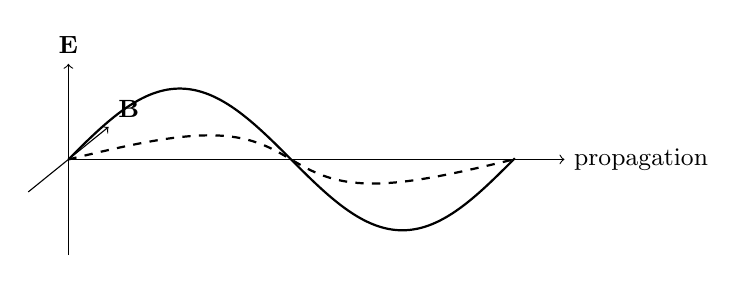
\begin{tikzpicture}[
  scale=0.9,
  x={(1cm,0cm)},
  y={(0cm,1cm)},
  z={(0.42cm,0.34cm)}
]
\draw[->] (0,0,0) -- (7,0,0) node[right] {\small propagation};
\draw[->] (0,-1.35,0) -- (0,1.35,0) node[above] {\small \(\mathbf E\)};
\draw[->] (0,0,-1.35) -- (0,0,1.35) node[above right] {\small \(\mathbf B\)};
\draw[thick,smooth,variable=\x,domain=0:6.3,samples=100]
  plot ({\x},{sin(\x r)},0);
\draw[thick,dashed,smooth,variable=\x,domain=0:6.3,samples=100]
  plot ({\x},0,{sin(\x r)});
\end{tikzpicture}
\caption{在电磁波中，电场与磁场相互垂直，并且都垂直于传播方向。}
\end{figure}

普通可见光的振荡快到远无法直接跟随其交变场。对于极长的无线电波，振荡则相应地更慢。无论哪种情形，同样的横波几何结构都会给出干涉。

\section{波长、周期与频率}

波长\(\lambda\)是一个空间距离：从振荡中的某一点出发，沿波移动，直到经过一个完整周期后同一相位再次出现。它以米、厘米或任何其他长度单位来量度。

现在站在某一位置不动，让波通过。完成一个完整周期所需的时间就是周期\(T\)。可见光的周期极短，大致为\(10^{-15}\,\mathrm{s}\)量级；波长越长对应周期越长，波长越短对应周期越短。

在一个周期内，波前进一个波长，因此速度为\(v\)的波满足
\begin{equation}
v=\frac{\lambda}{T}.
\end{equation}
水波和声波各有其传播速度。对于光，
\begin{equation}
c=\frac{\lambda}{T}.
\end{equation}
频率\(f\)是单位时间内的周期数：
\begin{equation}
f=\frac{1}{T}.
\end{equation}
因此
\begin{equation}
\lambda f=c.
\end{equation}
波长或频率中任意一个都决定另一个。

\begin{figure}[h]
\centering
\includegraphics[width=0.68\textwidth]{lecture_01_figure_03.png}
\caption{对于光波，\(f=1/T\)且\(\lambda f=c\)。}
\lectureframe{00:36:24}
\end{figure}

物理学家常用每秒弧度而非每秒完整周期来量度振荡速率。想象一个质点沿圆周做匀速运动。如果该点每秒完成\(f\)圈，而每圈包含\(2\pi\)弧度，则其角频率为
\begin{equation}
\omega=2\pi f,
\qquad
\frac{\omega}{2\pi}=f.
\end{equation}
目前这只是一个定义；它是否能减少\(2\pi\)因子的数目这一实际问题，稍后再谈。

将\(f=c/\lambda\)与\(\omega=2\pi f\)结合，得到
\begin{equation}
\omega=\frac{2\pi c}{\lambda},
\qquad
\omega\lambda=2\pi c.
\end{equation}
对于另一种波，\(c\)应替换为该波的传播速度。

\begin{figure}[h]
\centering
\includegraphics[width=0.68\textwidth]{lecture_01_figure_04.png}
\caption{在\(\omega=2\pi f\)下，光波满足\(\omega=2\pi c/\lambda\)。}
\lectureframe{00:39:10}
\end{figure}

电磁辐射构成连续谱。按波长从长到短排列，惯用名称为
\begin{equation}
\begin{aligned}
\text{radio}
&\longrightarrow \text{microwave}
\longrightarrow \text{infrared}
\longrightarrow \text{visible}\\
&\longrightarrow \text{ultraviolet}
\longrightarrow \text{X ray}
\longrightarrow \text{gamma ray}.
\end{aligned}
\end{equation}
可见光只占据一个狭窄区间。各命名区域之间的边界是约定性的，因此这里不需要精确的分界波长。无线电波可以极长；伽马辐射是电磁波谱中波长极短的一端。困难现在变得尖锐：伽马辐射在经典意义上是连续的场波，却被探测为离散的脉冲。

\section{离散到达与波概率}

辐射的热力学性质使普朗克和爱因斯坦得出结论：光必须按离散单元来处理。一个想象实验能把这一点讲得很生动，但它并不是关于实际历史发现路径的主张。

把一束光照射到屏幕上。在普通强度下，它形成一个看起来连续的亮斑。在光束中放入一个部分不透明的衰减器：亮斑变暗。反复增大衰减，单位时间内到达的光越来越少。最终外观发生变化。探测器记录到的不再是连续变暗的亮斑，而是孤立的事件。\footnote{这一示意图重建了讲课视频中在00:42:32与00:45:42之间展开的衰减实验。}

\begin{figure}[h]
\centering
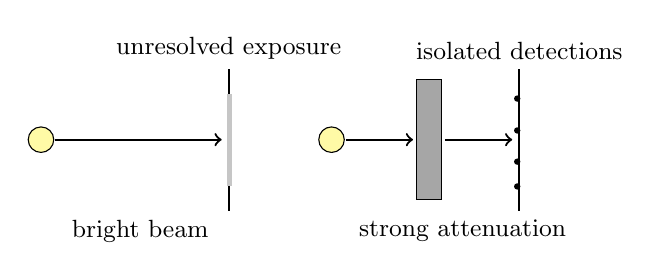
\begin{tikzpicture}[scale=0.9]
\begin{scope}
\draw[fill=yellow!35] (0,0) circle (0.18);
\draw[->,thick] (0.2,0) -- (2.55,0);
\draw[thick] (2.65,-1.0) -- (2.65,1.0);
\node[below] at (1.4,-1.0) {\small bright beam};
\end{scope}
\begin{scope}[xshift=4.1cm]
\draw[fill=yellow!35] (0,0) circle (0.18);
\draw[->,thick] (0.2,0) -- (1.15,0);
\draw[fill=gray!70] (1.2,-0.85) rectangle (1.55,0.85);
\draw[->,thick] (1.6,0) -- (2.55,0);
\draw[thick] (2.65,-1.0) -- (2.65,1.0);
\node[below] at (1.85,-1.0) {\small strong attenuation};
\end{scope}
\fill[gray!45] (2.62,-0.65) rectangle (2.70,0.65);
\foreach \y in {-0.66,-0.31,0.13,0.58}
  \fill (6.72,\y) circle (0.045);
\node[above] at (2.65,1.0) {\small unresolved exposure};
\node[above] at (6.75,1.0) {\small isolated detections};
\end{tikzpicture}
\caption{逐步衰减降低探测率，直到看起来连续的曝光分解为孤立的光子事件。}
\end{figure}

等待足够长的时间，这些事件就会累积成与原始团块相同的空间分布。因此，亮区是许多单个到达事件的未分辨总和。这个低强度实验是可以进行的，尽管它并不是最初激发光子假说的那个早期实验。爱因斯坦的光子提议源于热力学和光电方面的考虑；衰减实验提供了一种特别直接的方式来想象其后果。

现在在光束中放置两个孔径，并降低强度，直到光子一次一个地到达。每次探测都是一个局域化的信号。然而在多次探测之后，这些信号填充出干涉图样，包括亮带和暗带。离散的到达是随机的，但它们的概率分布正是波图样所预言的分布。经典波已经变成了一种支配概率的波。

因此，波和粒子并不是分配给自然界不同部分的两种独立实体。它们是同一个量子对象的两种表现。光不能被充分描述为仅仅是波或仅仅是粒子。

电子逆转了最初的惊奇。电子被接受为粒子，并且一次一个地到达探测器，但在孔径足够接近时，它们也会构建出干涉图样。{\proseunicodefont α}粒子比电子重约八千倍，也遵循同样的原理，尽管实验更难。干涉甚至已经在巴基球上被观察到：由六十个碳原子组成的分子，其排列大致像一个广义的足球。同样的原理预计甚至适用于保龄球，尽管这样的实验极其不切实际。讨论可以推向用病毒或活细胞进行的提议实验，作为越来越雄心勃勃的例子。理解波和粒子的描述如何相互契合需要量子力学；当前的任务是提取粒子物理学所需的光子性质。

\section{光子能量}

光子是光的离散、不可分割的单元。光携带能量---阳光加热吸收物体---所以每个光子必须携带能量。单色波具有确定的波长和角频率，其中的每个光子都有
\begin{equation}
E_\gamma=\hbar\omega.
\end{equation}
试图把连续波想象成一个小型机械点集是误导性的。确定的是实验组合：局域化探测以波支配的分布发生，而能量以不可分割的单元到达。

由于
\begin{equation}
\omega=\frac{2\pi c}{\lambda},
\end{equation}
较短的波长意味着较大的角频率，因此每个光子中的能量更多：
\begin{equation}
\lambda\downarrow
\quad\Longrightarrow\quad
\omega\uparrow
\quad\Longrightarrow\quad
E_\gamma\uparrow.
\end{equation}
单个无线电光子的能量非常小。然而，无线电束可以通过包含非常多的光子来携带巨大的总能量。对于包含\(n\)个光子的单色脉冲，
\begin{equation}
E_{\text{pulse}}=n\hbar\omega,
\qquad
n=0,1,2,\ldots.
\end{equation}
总量可能很大，但它仍然是单光子能量的整数倍。

这个关系指向了将支配其余讨论的实际问题。为什么必须建造越来越大的机器来观察越来越小的东西？为什么不用小机器来研究小物体？答案的前一半已经存在：分辨更小的结构需要更短的波长，而更短波长的量子携带更大的能量。

\section{静能量与不变质量}

粒子物理学将量子力学与相对论结合起来。光子关系\(E_\gamma=\hbar\omega\)提供了量子方面；相对论中相应的基本事实是
\begin{equation}
E_{\mathrm{rest}}=mc^2.
\end{equation}
这个限定很重要。较早的论述将\emph{静质量}与依赖于速度的\emph{动质量}区分开来。现代术语用\emph{质量}来表示物体的不变质量。运动改变的是它的能量，而不是它的质量。每个电子都有相同的质量，无论其运动状态如何，而电子的能量在加速时会增加。因此，\(E=mc^2\)在这个形式下，是物体作为一个整体在其中静止的参考系中有质量物体的能量。

物体不必在内部静止不动。一箱气体可以在秤上静止不动，而其分子向各个方向快速运动。这些内部运动的能量是完整箱子静能量的一部分。从冷箱子开始，测量其质量，然后在保持箱子本身静止的同时加入热能。它的静质量变化为
\begin{equation}
\Delta m=\frac{\Delta E_{\mathrm{internal}}}{c^2}.
\end{equation}
它的重量和惯性随其质量增加。对于普通的箱子，即使温度大幅升高，这种效应在普通秤上也小得无法察觉；效应的微小并不改变原理。

一个更鲜明的例子使用电子和正电子。它们具有完全相等的质量和相反的电荷。如果它们最初处于静止状态并发生湮灭，光子会带走能量：
\begin{equation}
e^-+e^+\longrightarrow \text{photons}.
\end{equation}
初始能量为
\begin{equation}
E_{\mathrm{initial}}=2m_e c^2,
\end{equation}
而这份能量不可能消失。一对粒子只产生极微小的量，因此即使要加热一杯咖啡也需要数量庞大的粒子对，但单个湮灭事件直接展示了这种转换。

因此，对于静止的物体，质量和能量是同一物理量以不同单位表达的结果。因子\(c^2\)是惯用质量单位与能量单位之间的换算因子，正如一个数值因子将米换算为厘米。

\begin{classroomqa}
\lecturetimestamp{01:04:39}
\audiencequestion{将质量转化为释放的能量需要一个机制吗？}
\lecturerresponse{是的，需要一个物理机制，但守恒定律已经约束了它的结果。即使在描述微观湮灭机制之前，初始的电子--正电子能量也必须在某处重新出现。因此，能量守恒可以在没有详细描述相互作用的情况下确定答案的重要部分。}
\end{classroomqa}

\section{量纲与单位的选择}

在SI单位中，光速是一个非常大的数，而普朗克常数是一个非常小的数。后者的微小性已由光子关系式暗示：可见光的角频率极大，而单个光子的能量极小，因此\(E_\gamma=\hbar\omega\)在这些单位中要求\(\hbar\)取一个小的数值。在数量级层面上，
\begin{equation}
c\sim 10^8\ \mathrm{m\,s^{-1}},
\qquad
\hbar\sim 10^{-34}\ \mathrm{J\,s}.
\end{equation}
\editorialnote{仅保留讲座中所述的数量级，因为最后的板书数字不清晰。}
单位至关重要：两个常数都不仅仅是裸小数。由于能量具有量纲
\begin{equation}
[E]=M L^2 T^{-2},
\end{equation}
且\(E_\gamma=\hbar\omega\)，其中\([\omega]=T^{-1}\)，普朗克常数具有量纲
\begin{equation}
[\hbar]=[E]T=M L^2 T^{-1}.
\end{equation}

称\(c\)大、\(\hbar\)小，已经预设了单位的选择。以英尺每小时测量速度得到的\(c\)数值不同于以米每秒测量。以光年每年或光秒每秒为单位，光速恰好为一。对质量、长度和时间单位进行适当的协调选择，同样可以使\(\hbar=1\)。

熟悉的单位制是继承下来的约定，而非自然界的特权特征。一英里包含5280英尺，一英石包含十四磅，马以掌宽来度量，功率可以用马力来度量。公制单位更为系统，但其尺度仍然是人为选择。基础物理学中没有任何东西单独挑出米、秒或千克。

长度、时间和质量提供了三个独立的基本单位选择：
\begin{equation}
L,\qquad T,\qquad M.
\end{equation}
其他力学单位可以由它们构建。有用的选择取决于问题。太阳质量在天体物理学中很方便；质子质量在核物理学中可能很方便；光年和年使相对论天体物理公式变得紧凑。有了三个独立选择，人们可以为三个独立的量纲常数赋予方便的数值。天体物理学、原子物理学和粒子物理学不必做出相同的选择。

对于粒子物理学，两个特别有用的约定是
\begin{equation}
c=1,
\qquad
\hbar=1.
\end{equation}
对于剩余的单位，没有可比拟的、同样突出的粒子质量。人们可以宣布质子质量、希格斯玻色子质量或{\proseunicodefont μ}子质量为一，但那只会使一个庞大家族中的一员享有特权。

那么，为什么选择\(c\)和\(\hbar\)呢？第一个答案可能是它们出现在许多方程中。出现频率并不足够：质子质量也出现在许多方程中，质子的尺寸也是如此。\(c\)和\(\hbar\)的独特之处在于它们的普适性。

常数\(c\)和\(\hbar\)是不同的。速度\(c\)约束每一个物理物体：有质量的物体可以接近它，但不能被加速穿过它。普朗克常数通过数量级不确定性关系
\begin{equation}
\Delta x\,\Delta p\gtrsim\hbar.
\end{equation}
约束每一个量子物体。这两个陈述都没有单独挑出某一特定种类的粒子。正是这种普适性使\(c=1\)和\(\hbar=1\)成为自然的约定。

质子没有提供可比拟的普适尺度。它只是众多物体中的一个。将质子质量设为一，其基础地位并不比将铷原子质量设为一更高；电子、希格斯玻色子和{\proseunicodefont μ}子也带来同样的困难。

电荷暗示着另一种普适的量，但在\(c\)和\(\hbar\)被归一化之后，具有物理意义的电磁耦合是无量纲的。改变单位可以使量纲常数在电磁公式中四处移动；它不能改变一个真正的无量纲耦合。

引力提供了一种有量纲的普适常数。在牛顿形式中，两个质量之间力的大小为
\begin{equation}
F=G\frac{m_1m_2}{r^2}.
\end{equation}
每个质量都参与引力作用，而电中性的物体则不必参与电力。因此\(G\)具有所需的普适性。然而，对于普通粒子物理而言，它是一种糟糕的实用归一化，因为已知基本粒子之间的引力在所讨论的计算中可以忽略不计。

\begin{classroomqa}
\lecturetimestamp{01:20:34}
\audiencequestion{简单地摒弃\(G\)是否合理？在极高能量下，基本粒子可能不会以所假设的方式遵循经典引力。}
\lecturerresponse{单个粒子确实会响应地球的引力场：单个粒子会在该场中下落。一个基本粒子对另一个基本粒子的引力影响尚未被直接测量，因此普适性假设在那个层面上是可以被质疑的。将\(G\)排除在外的直接原因是实用性的而非绝对的：引力对普通粒子物理实验和方程的贡献可以忽略不计。}
\end{classroomqa}

\begin{classroomqa}
\lecturetimestamp{01:22:01}
\audiencequestion{能否用电力相互作用代替引力作为第三种设定单位的约定？}
\lecturerresponse{可以。人们可以选择电磁单位，使电荷或库仑定律中出现的常数被归一化。这样的约定确实在使用。电子相互排斥而非吸引，但那个符号并不妨碍这一选择。它只是并非此处所采用的约定。}
\end{classroomqa}

\begin{classroomqa}
\lecturetimestamp{01:23:06}
\audiencequestion{一旦\(c\)和\(\hbar\)被设为一，电荷就是无量纲的吗？}
\lecturerresponse{是的。与电荷平方相关的一个无量纲量度约为\(1/137\)。确切的约定以及那个数的含义可以推迟讨论；这里的要点在于它是无量纲的。}
\end{classroomqa}

\begin{classroomqa}
\lecturetimestamp{01:23:37}
\audiencequestion{能否选择库仑常数作为第三个被设为一的常数？}
\lecturerresponse{它可以被吸收进电磁单位约定中。那种选择不能把无量纲耦合\(1/137\)变成一，因为改变单位不能改变一个无量纲的数。此处并不声称采用那种约定有什么特别的好处。}
\end{classroomqa}

\section{自然单位方程与参考系}

在\(c=1\)下，有质量物体的静止能量关系变为
\begin{equation}
E_{\mathrm{rest}}=m.
\end{equation}
在\(\hbar=1\)下，光子关系变为
\begin{equation}
E_\gamma=\omega.
\end{equation}
每当需要以常规单位表示的数值大小时，这些常数都可以被恢复。

\begin{figure}[h]
\centering
\includegraphics[width=0.72\textwidth]{lecture_01_figure_05.png}
\caption{在\(c=1\)的单位下，静止的有质量物体的静止能量为\(E=m\)。}
\lectureframe{01:25:40}
\end{figure}

这些公式看起来相似，但含义不同。在\(E_{\mathrm{rest}}=m\)中，\(E\)是有质量物体的静止能量。光子没有质量，不能被带到静止，因此它的能量不是静止能量。关系式\(E_\gamma=\omega\)给出的是一个运动的、无质量量子的能量。

\begin{classroomqa}
\lecturetimestamp{01:26:07}
\audiencequestion{当静止总是相对于某物而言，而实验室本身并非绝对静止时，\emph{静止}意味着什么？}
\lecturerresponse{静止是相对于所选参考系定义的。如果一个杯子相对于实验室是静止的，那么在该实验室参考系中，当\(c=1\)时，它的能量就是它的质量，没有整体的动能贡献。另一个从杯子旁经过的观察者则会赋予它动能。不同的观察者通常会给同一物体或光子赋予不同的能量；能量依赖于参考系，不需要任何绝对静止的断言。}
\end{classroomqa}

现在可以重新考虑角频率约定。写成\(E_\gamma=\hbar\omega\)很紧凑，但\(\omega=2\pi f\)此前插入了一个\(2\pi\)的因子。

\begin{classroomqa}
\lecturetimestamp{01:28:13}
\audiencequestion{为什么使用以弧度每秒为单位的角频率\(\omega\)，而不是表面上更简单的每秒完整周期数？}
\lecturerresponse{这一选择部分出于历史原因，而数学上的答案与其说是直接的，不如说是实用的。这里给出的答案是尝试性的：用\(f\)写一次相关方程，再用\(\omega\)写一次，然后看哪种约定留下的\(2\pi\)因子更少。\(2\pi\)的因子无法在所有地方都消失。也曾提出过与复指数记号的可能联系，但这里并未展开。}
\end{classroomqa}

\begin{classroomqa}
\lecturetimestamp{01:29:51}
\audiencequestion{两个粒子能否被加速到它们之间的引力相互作用变得重要？}
\lecturerresponse{原则上可以。实际上，目前的加速器距离那个区域极其遥远。答案还取决于“粒子”指的是什么：宏观的引力物体并不是这里所讨论的基本粒子情形。}
\end{classroomqa}

\begin{classroomqa}
\lecturetimestamp{01:30:27}
\audiencequestion{什么可以作为正电子的来源？}
\lecturerresponse{高能碰撞可以产生正电子。某些核过程和衰变也会产生正电子。}
\end{classroomqa}

\begin{classroomqa}
\lecturetimestamp{01:30:53}
\audiencequestion{普朗克时间和普朗克距离是这里使用的自然单位吗？}
\lecturerresponse{不是。普朗克单位出现在\(G\)、\(c\)和\(\hbar\)都被取为1时。由此得到的普朗克长度远小于普通粒子物理的长度尺度，因此在这里是一种不方便的度量标准。当引力、量子力学和相对论都同时重要时，例如在黑洞物理、宇宙学或量子引力中，这样的单位才是自然的。当引力可以忽略时，只把\(c\)和\(\hbar\)取为1更有用。}
\end{classroomqa}

\section{动量、光与分辨率}

下一个基本概念是动量。静止的物体没有动量，尽管它具有非零的静止能量\(mc^2\)。一旦它运动起来，通常就携带动量。动量在碰撞中守恒，正如能量守恒一样：当两个物体碰撞时，碰撞前后的总矢量动量相同。任何受守恒定律约束的东西都值得特别关注。

动量是矢量：它指向运动方向。对于非相对论性物体，
\begin{equation}
\mathbf p=m\mathbf v.
\end{equation}
这不是一般的相对论公式，不能直接应用于光。

然而光既携带能量，也携带动量。普通光产生的推力如此之小，以至于其动量很难被注意到，但强激光脉冲可以传递可观的冲量。例如，利弗莫尔的大型激光器可以用其辐射携带的动量将物质向内驱动。

考虑一个准直得足够好、其光线几乎沿一个轴传播的脉冲。真实光束可能有一定的角展宽，其中各部分沿略微不同的方向传播，但对于理想的准直光束，动量沿光束方向，其大小为
\begin{equation}
p=\frac{E}{c},
\qquad\text{or equivalently}\qquad
E=cp.
\end{equation}
这里把这一关系当作相对论事实来接受，而不是加以证明。下面的量纲检验只是确认其单位与普通动量的单位一致：
\begin{equation}
\left[\frac{E}{c}\right]
=
\frac{M L^2 T^{-2}}{L T^{-1}}
=
M L T^{-1}
=
[m v]
=
[p].
\end{equation}
这种量纲比较并没有给光赋予静止质量。光子质量为零；它携带动量，是因为它携带能量并以\(c\)运动。

\(\mathbf p\)的方向就是传播方向。其大小通常难以探测，因为\(c\)出现在分母中。光束可以通过加热或蒸发物质轻易地显露其能量，而它的机械推力则小得多。然而，只要强度足够大，这种推力就可以变得很大。

对于一个光子，
\begin{align}
p_\gamma
&=\frac{E_\gamma}{c}\\
&=\frac{\hbar\omega}{c}.
\end{align}
要用波长来表示它，需仔细回到波的关系式。由于
\begin{equation}
f\lambda=c,
\qquad
\omega=2\pi f,
\end{equation}
正确的关系是
\begin{equation}
\omega\lambda=2\pi c,
\qquad
\omega=\frac{2\pi c}{\lambda}.
\end{equation}
如果不把定义写出来，\(2\pi\)这个因子很容易弄反。从\(f\lambda=c\)和\(f=\omega/(2\pi)\)重新出发即可解决这个问题：
\begin{equation}
\frac{\omega}{2\pi}\lambda=c
\quad\Longrightarrow\quad
\omega\lambda=2\pi c.
\end{equation}
现在代入得到
\begin{align}
p_\gamma
&=\frac{\hbar}{c}\frac{2\pi c}{\lambda}\\
&=\frac{2\pi\hbar}{\lambda}\\
&=\frac{h}{\lambda}.
\end{align}

\begin{classroomqa}
\lecturetimestamp{01:42:38}
\audiencequestion{\(2\pi\hbar\)等于\(h\)吗？}
\lecturerresponse{是的。根据定义\(h=2\pi\hbar\)，所以\(p_\gamma=2\pi\hbar/\lambda\)与\(p_\gamma=h/\lambda\)相同。无论选择哪种频率约定，\(2\pi\)的因子都会在某个地方重新出现。}
\end{classroomqa}

波长越短，光子动量越大。射电光子的波长非常长，动量极小。伽马射线光子的波长非常短，带来的反冲大得多。一个光子仍然只给出很小的宏观冲量，但其动量远大于射电光子。其能量也更大，因为\(E_\gamma=cp_\gamma\)。

这一关系解释了为什么更小的物体需要更大的机器。用比人的头部长得多的波长拍摄的照片只能显示一片模糊。要分辨面部特征，波长必须短于头部。要分辨一根头发，波长必须与头发粗细相当或更小。要分辨原子的结构，探测波长不得大于原子：
\begin{equation}
\lambda_{\mathrm{probe}}\lesssim
\text{size of the structure to be resolved}.
\end{equation}
因此，更小的结构需要更短的波长，而更短的波长需要更大的动量和能量。探测粒子不必是光子；其他种类的高能粒子也遵循同样的波长与动量之间的量子联系。产生它们需要加速器将越来越多的能量转移给每个粒子。\(p_\gamma=h/\lambda\)和\(E_\gamma=\hbar\omega\)这一对关系承载了这一论证：提高探测能量会增大其动量并缩短其波长。

这在大约一个世纪里一直是粒子物理学反复出现的模式：更高的能量、更大的动量、更短的波长，以及更精细的空间分辨率。

\begin{classroomqa}
\lecturetimestamp{01:46:57}
\audiencequestion{波长是否存在理论上的下限？}
\lecturerresponse{可能存在。在普朗克长度附近预期会出现新东西，但答案仍是初步的。如果空间分辨率在那里触底，那么该尺度仍比大型强子对撞机所探测的距离低约十七个数量级，因此目前的实验距离它仍然极其遥远。}
\end{classroomqa}

同样的推理链条暗示了加速器的尺度与其所能分辨的尺度之间存在粗略的联系。

\begin{classroomqa}
\lecturetimestamp{01:48:02}
\audiencequestion{波长，或者说被分辨的尺寸，是否与加速器的尺寸大致成反比？}
\lecturerresponse{大致如此，前提是加速粒子的最大电场以及用于引导粒子的磁场由现有装置所固定。加速梯度是单位长度上的能量增益。对于长度为\(L\)、梯度\(\mathcal G\)近似固定的直线加速器，
\[
E_{\mathrm{beam}}\sim \mathcal G L.
\]
在极端相对论能量下，可分辨的波长与能量成反比，因此增加直线加速器的长度会以大致反比的因子改善分辨率。这只是一个启发性的标度关系，并非精确定律。环形机器允许同一装置被反复穿越，但被加速的电荷在偏转时会辐射并损失能量。}
\end{classroomqa}

\begin{classroomqa}
\lecturetimestamp{01:49:47}
\audiencequestion{要到达普朗克长度，加速器必须有多大？}
\lecturerresponse{按照这一粗略标度，它必须比欧洲核子研究组织的加速器长约十七个数量级。这不是宇宙的大小，但大致是星系尺度。}
\end{classroomqa}

\begin{classroomqa}
\lecturetimestamp{01:50:09}
\audiencequestion{最高能量的宇宙射线的能量与对撞机能量相比如何？}
\lecturerresponse{单个宇宙射线可以具有远高于实验室的能量。为了进行数值比较，取一个实验室能量约为\(10^{21}\,\mathrm{eV}=10^{12}\,\mathrm{GeV}\)的极端宇宙射线。但宇宙射线撞击的是在实验室中静止的靶，而对撞机则将两束高能束流迎头相撞。更重要的是，有用的实验需要通量：许多粒子以及许多控制良好的碰撞。孤立的宇宙射线可能错过相关的靶，或者产生一个几乎无法推断出什么的事件。一个刻意夸张的石油当量估计认为，运行一台有用的星系尺度加速器所需的供应约为每秒一百万亿桶石油。其目的是表明，足够的碰撞统计量至少会和加速器的长度一样构成严重障碍。}
\end{classroomqa}

\editorialnote{石油当量估计在来源中不一致。它先被表述为，随后又被重复为约每秒\(10^{14}\)桶；后来的一次重述给出每秒\(10^{11}\)桶。两种尺度都被保留，而不是被悄然调和。}

这些是真实的距离尺度，而不仅仅是形式上的尺度。实际的难题在于，如何在不建造星系尺度加速器并提供其荒诞功率的情况下探测它们。

\begin{classroomqa}
\lecturetimestamp{01:52:55}
\audiencequestion{LHC的能量应当如何与能量为\(10^{12}\,\mathrm{GeV}\)的宇宙射线相比较？}
\lecturerresponse{对于实验室能量为\(E_{\mathrm{lab}}\)的超相对论性入射粒子撞击质量为\(m_{\mathrm{target}}\)的固定靶的情形，质心能量在参数上表现为
\[
E_{\mathrm{cm}}\simeq
\sqrt{2m_{\mathrm{target}}c^2E_{\mathrm{lab}}}.
\]
\editorialnote{所展示的固定靶表达式明确给出了对话中所述的平方根标度关系。}
因此，在靶质量保持固定的情况下，有用的碰撞能量仅随入射粒子能量的平方根增长。于是，能量为\(10^{12}\,\mathrm{GeV}\)的宇宙射线在数量级层面上对应于每束约为\(10^6\,\mathrm{GeV}\)的对撞束能量，而不是每束\(10^{12}\,\mathrm{GeV}\)。宇宙射线仍然可以超过地面对撞机的能量，但其极低的通量使得系统性的受控实验不切实际。}
\end{classroomqa}